\documentclass{article}
\usepackage{pgfplots}
\pgfplotsset{compat=1.17}

\begin{document}

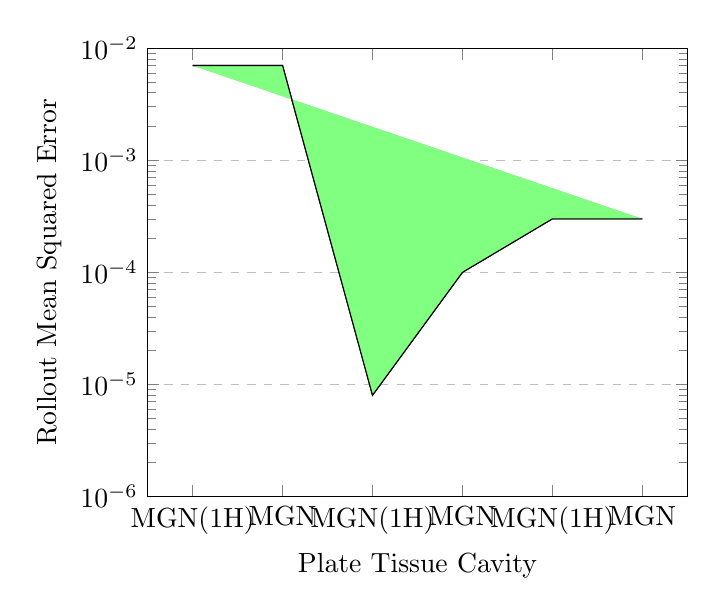
\begin{tikzpicture}
    \begin{axis}[
        ymode=log,
        log basis y={10},
        ymin=1e-6, ymax=1e-2,
        xlabel={Plate Tissue Cavity},
        ylabel={Rollout Mean Squared Error},
        xtick=data,
        xticklabels={MGN(1H), MGN, MGN(1H), MGN, MGN(1H), MGN},
        ymajorgrids=true,
        grid style=dashed,
    ]
        \addplot[fill=gray!50] coordinates {
            (1, 7e-3) (2, 7e-3) (3, 8e-6) (4, 1e-4) (5, 3e-4) (6, 3e-4)
        };
        \addplot[fill=green!50] coordinates {
            (1, 7e-3) (2, 7e-3) (3, 8e-6) (4, 1e-4) (5, 3e-4) (6, 3e-4)
        };
    \end{axis}
\end{tikzpicture}

\end{document}